\chapter[Estrutura]{Estrutura}

  \begin{figure}[H]
    \centering
    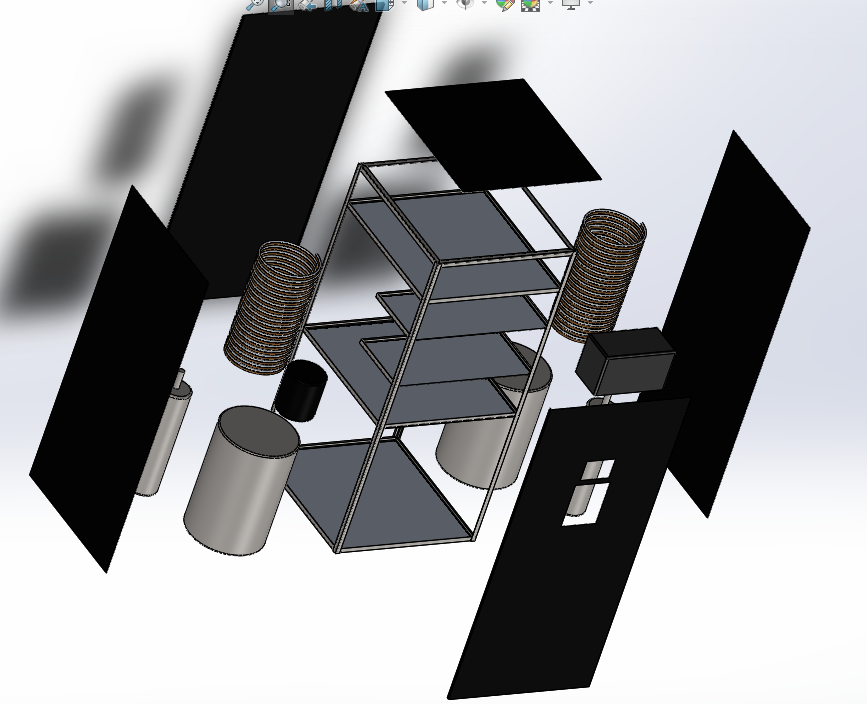
\includegraphics[scale= 0.4]{figuras/estrutura/Vista-explodida.png}
    \caption{Vista Explodida. Fonte: Própria.}
    \label{modelagem}
  \end{figure}

  \section[Levantamento dos esforços a serem levantados]{Levantamento dos esforços a serem levantados}

  Após a realização do packaging, começaram os trabalhos de integração com os outros subsistemas para 
  levantamento de requisitos. Após algumas reuniões foi verificado que a estrutura deveria ser capaz 
  de suportar o peso de dois barris de chopp de 67,4Kg cada e dois cilindros de CO2 de 20kg 
  no primeiro nível. O segundo nível suportaria todo o sistema de refrigeração e alimentação 
  do circuito elétrico da máquina que pesaria no total em torno de 50Kg e o terceiro nível 
  seria o reservatório dos copos.

  Entre o segundo e terceiro níveis existem dois subníveis que acomodam toda parte eletrônica e 
  de automação da máquina, como haspberrys, um motor de passo e algumas placas de circuito. 

  \begin{figure}[H]
    \centering
    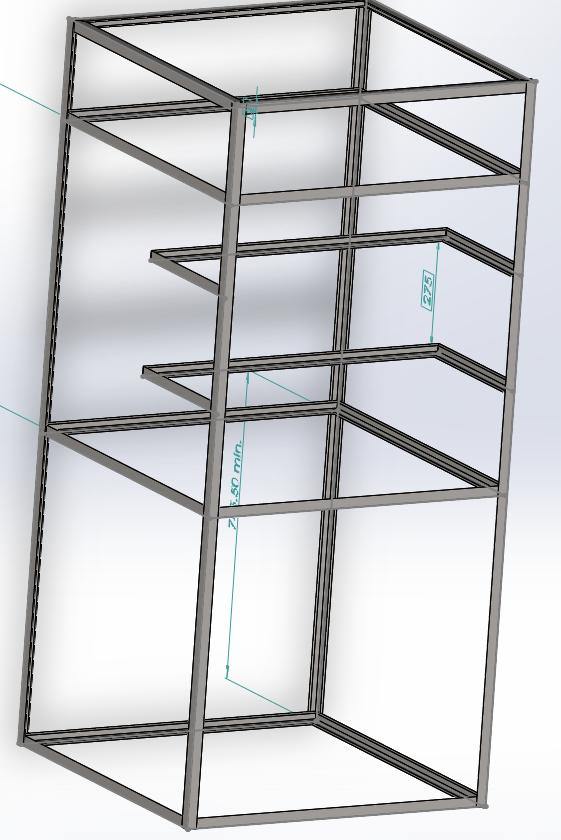
\includegraphics[scale= 0.4]{figuras/estrutura/frame-principal.png}
    \caption{Frame Principal. Fonte: Própria.}
    \label{modelagem}
  \end{figure}

  Segue abaixo algumas informações dos componentes mais pesados e de maior influência nos esforços suportados:

  \begin{itemize}
    \item \textbf{Barril:}
    \subitem  Peso: 67.4 \textit{Kg}
    \subitem  Altura: 740 \textit{mm}    
    \subitem  Diâmetro: 680 \textit{mm}
    
    \item \textbf{Sistema de refrigeração e alimentacão:}
    \subitem Peso: 50 \textit{Kg}
    \subitem Altura máxima: 750 \textit{mm}
  \end{itemize}

  Foi verificado que os níveis que suportariam a maior parte dos esforços seriam o primeiro e o segundo. 
  Sendo que o primeiro teria de suportar aproximadamente 1800N (680 de cada barril e 200N de cada 
  cilindro de CO2) e o segundo 500N (referente ao peso total de todos os componentes).
  
  \section[Simulação]{Simulação}

  \begin{figure}[H]
    \centering
    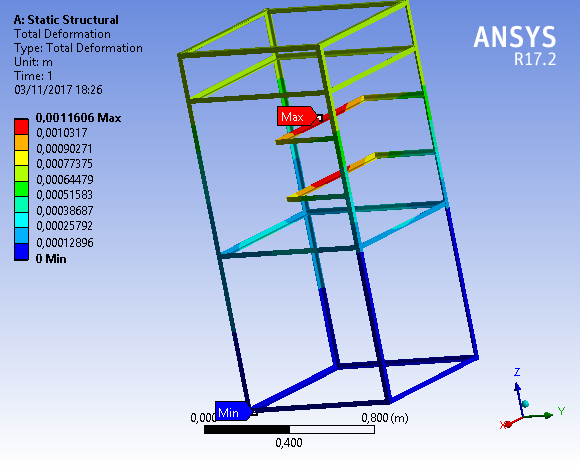
\includegraphics[scale= 0.8]{figuras/estrutura/deformacao-frame.png}
    \caption{Deformação Frame. Fonte: Própria.}
    \label{modelagem}
  \end{figure}

  As simulações do frame e das chapas foram feitas em separado. Para realizar as simulações
  iniciais foi utilizado o módulo de análise estrutural do Solidworks, pela praticidade e 
  rapidez de implementação de um modelo inicial. 

  Durante o projeto tudo foi passado para o software Ansys, que gerou resultados mais completos 
  e refinados, mas confirmando a análise prévia simplificada.

  Após a simulação do design inicial verificou-se que o frame feito com perfis L de aço 1020 
  suportaria os esforços sem maiores problemas.
  
  \begin{figure}[H]
    \centering
    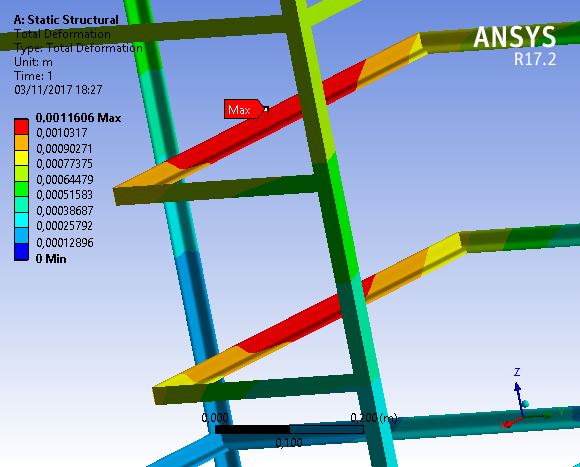
\includegraphics[scale= 0.6]{figuras/estrutura/deformacao-local.png}
    \caption{Deformação Local. Fonte: Própria.}
    \label{modelagem}
  \end{figure}
 
  \begin{figure}[H]
    \centering
    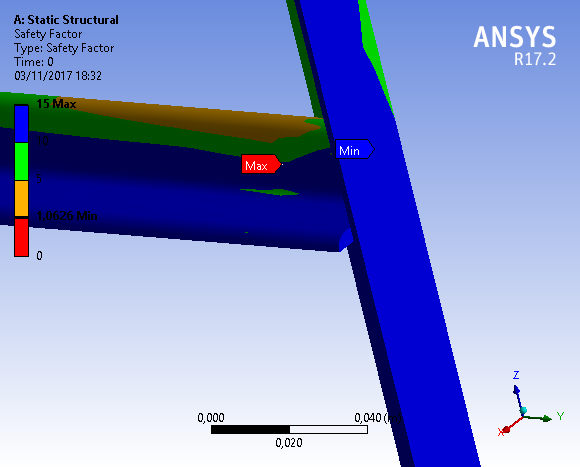
\includegraphics[scale= 0.6]{figuras/estrutura/fator-de-seguranca.png}
    \caption{Fator de Segurança. Fonte: Própria.}
    \label{modelagem}
  \end{figure}

  \begin{figure}[H]
    \centering
    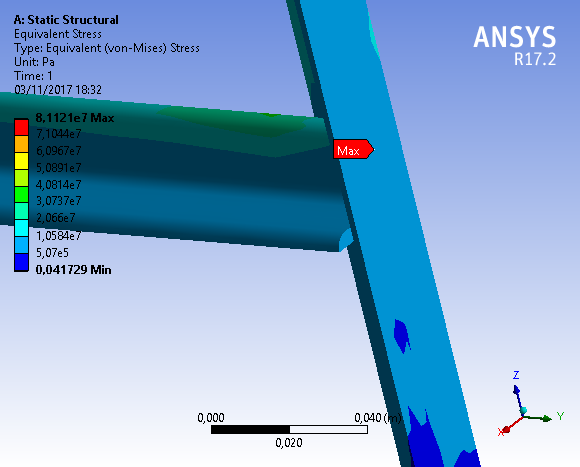
\includegraphics[scale= 0.6]{figuras/estrutura/tensao-local.png}
    \caption{Tensão Local. Fonte: Própria.}
    \label{modelagem}
  \end{figure}

  \begin{figure}[H]
    \centering
    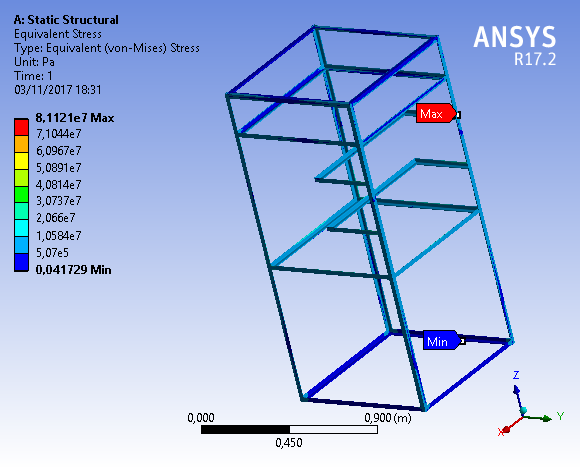
\includegraphics[scale= 0.6]{figuras/estrutura/tensao.png}
    \caption{Tensão. Fonte: Própria.}
    \label{modelagem}
  \end{figure}

  No que diz respeito às chapas de alumínio que formam as bases dos níveis, 
  percebeu-se que apesar da não ocorrência de escoamento ou ruptura do material, 
  a deflexão da chapa no primeiro nível estava excessiva (Aproximadamente 8mm de deflexão máxima), 
  de forma que comprometeria a qualidade do produto e de seu funcionamento.

  Foi decidido que o primeiro nível não seria feito com chapa de alumínio como decidido 
  anteriormente mas sim, com aço. Houve a opção de apenas aplicar uma treliça a este nível e 
  usar uma chapa de alumínio mais espessa porém o custo ficou muito elevado.

  A solução final foi aplicar treliças no primeiro e segundo níveis e usar chapas mais finas 
  (2mm ante 4mm que era usado no projeto inicial). Esta solução foi a que gerou a melhor relação 
  entre peso, custo e resistência mecânica (A deflexão máxima passou a ser de aproximadamente 2mm).

  \begin{figure}[H]
    \centering
    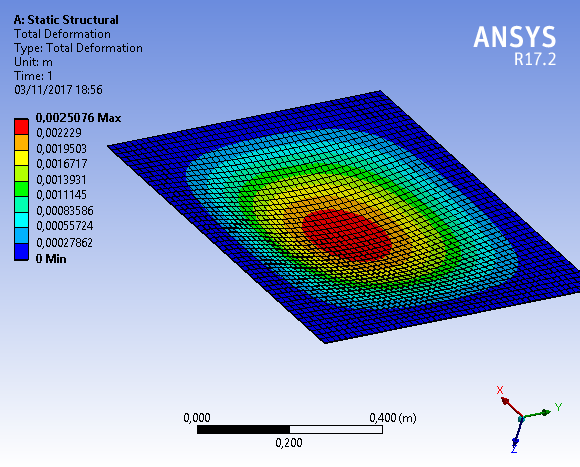
\includegraphics[scale= 0.6]{figuras/estrutura/deformacao-da-chapa.png}
    \caption{Deformação da chapa após redimensionamento. Fonte: Própria.}
    \label{modelagem}
  \end{figure}

  Os demais níveis foram feitos com chapa de alumínio como pensado anteriormente, 
  o que contribuiu para que o peso da estrutura não fosse muito elevado (aproximadamente 70kg).
  
  \section[Fabricação]{Fabricação}

  A fabricação foi pensada desde início, visando sempre simplicidade, 
  para que o projeto seja facilmente executável.

  Tudo começou pelo corte dos perfis em L. Na primeira etapa foram feitos os cortes 
  visando apenas acertar os comprimentos necessários para compor cada parte da estrutura. 
  Na segunda foram feitos cortes em 45 graus para facilitar o encaixe e melhorar o acamento.
  
  \begin{figure}[H]
    \centering
    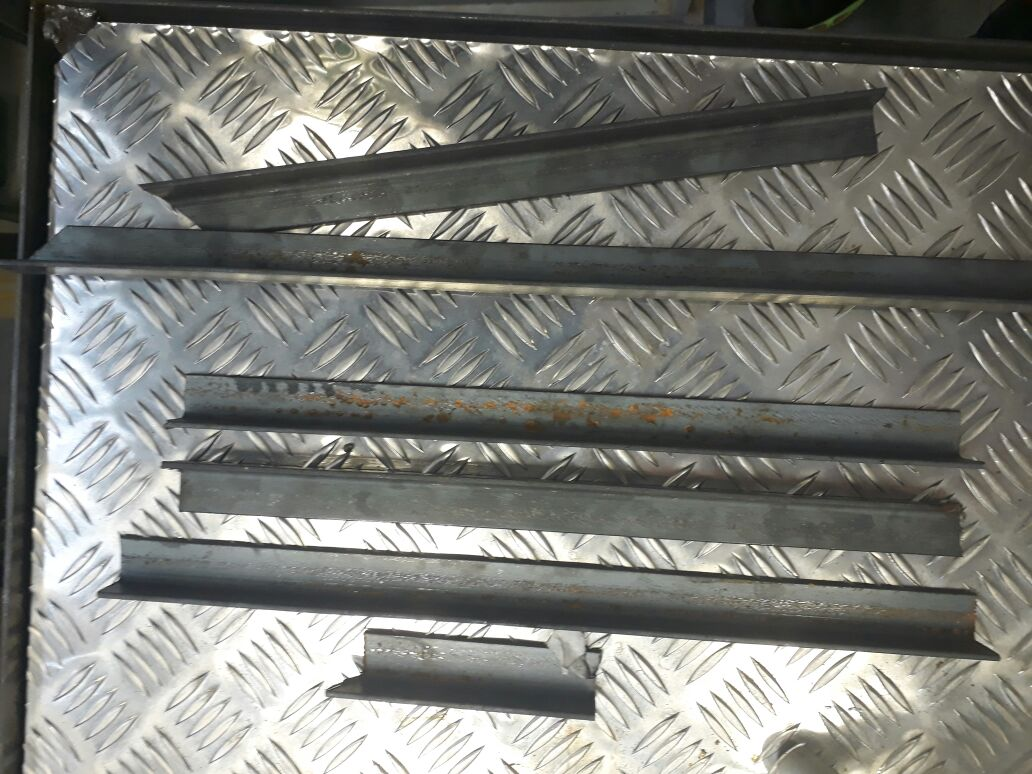
\includegraphics[scale= 0.3]{figuras/estrutura/perfis-cortados.jpg}
    \caption{Perfis Cortados. Fonte: Própria.}
    \label{modelagem}
  \end{figure}

  \begin{figure}[H]
    \centering
    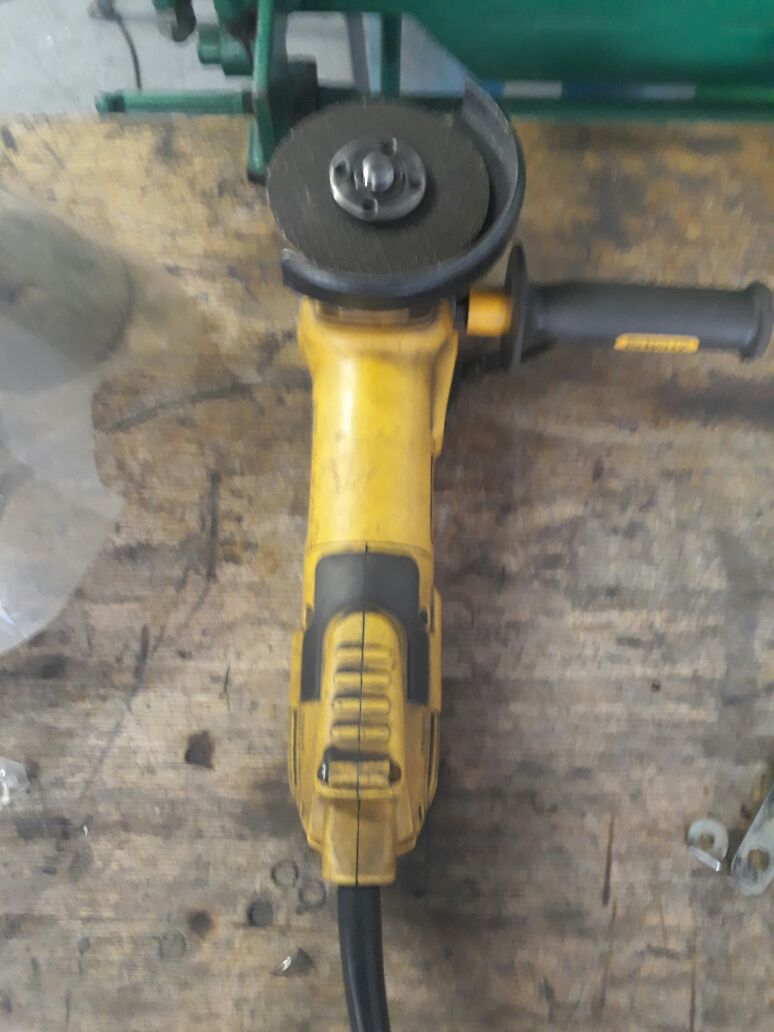
\includegraphics[scale= 0.3]{figuras/estrutura/esmerilhadeira.jpg}
    \caption{Esmerilhadeira usada para acabamento dos cortes. Fonte: Própria.}
    \label{modelagem}
  \end{figure}

  \begin{figure}[H]
    \centering
    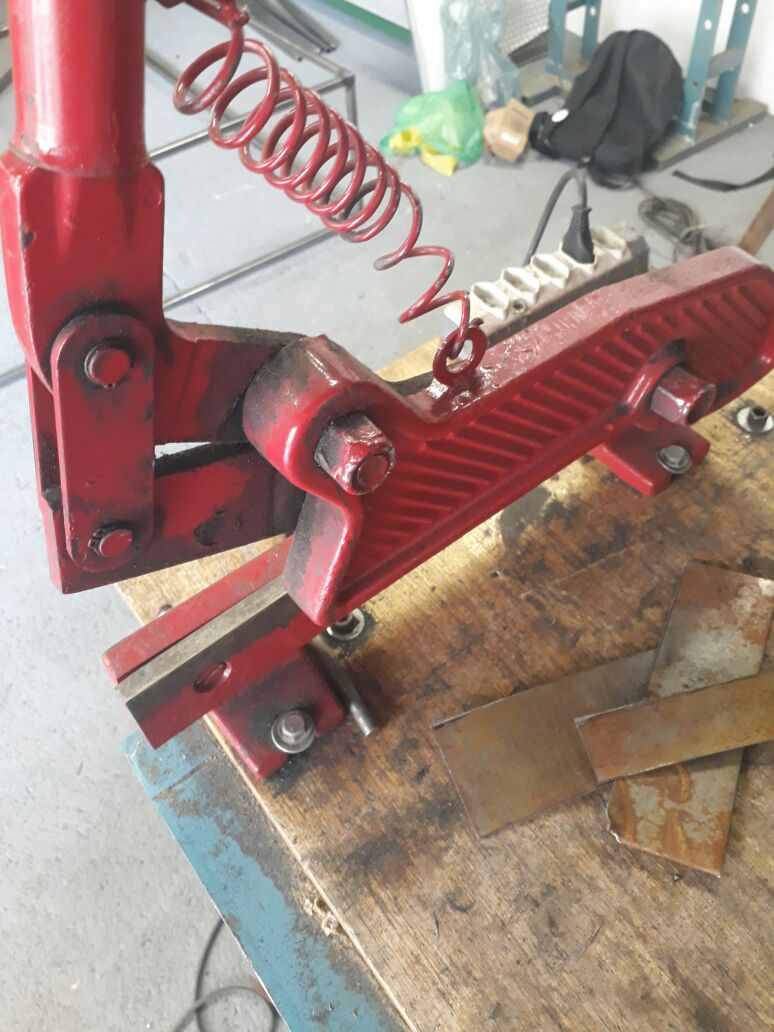
\includegraphics[scale= 0.3]{figuras/estrutura/guilhotina.jpg}
    \caption{Guilhotina usada no corte de chapas. Fonte: Própria.}
    \label{modelagem}
  \end{figure}

  Após toda a fase de corte foi iniciado o processo de soldagem das bases quadradas do frame. 
  O processo utilizado foi o MIG, devido principalmente à facilidade de acesso ao equipamento 
  e da boa qualidade referente ao resultado final. 

  \begin{figure}[H]
    \centering
    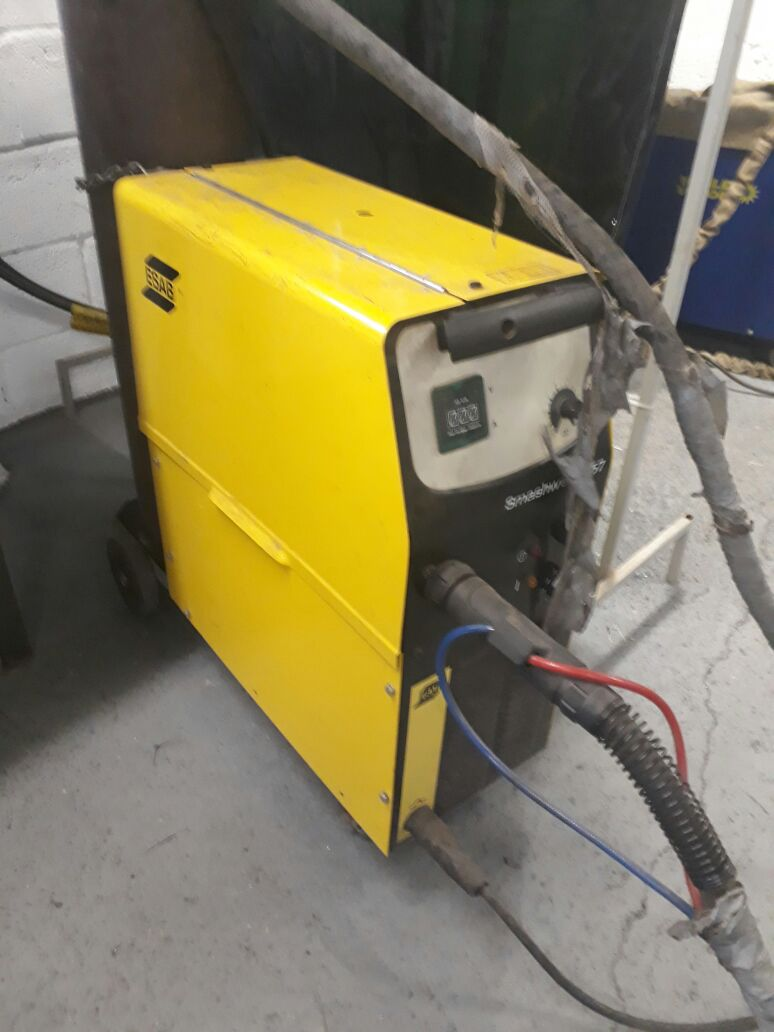
\includegraphics[scale= 0.2]{figuras/estrutura/maquina-soldagem.jpg}
    \caption{Maquina para soldagem MIG. Fonte: Própria.}
    \label{modelagem}
  \end{figure}

  \begin{figure}[H]
    \centering
    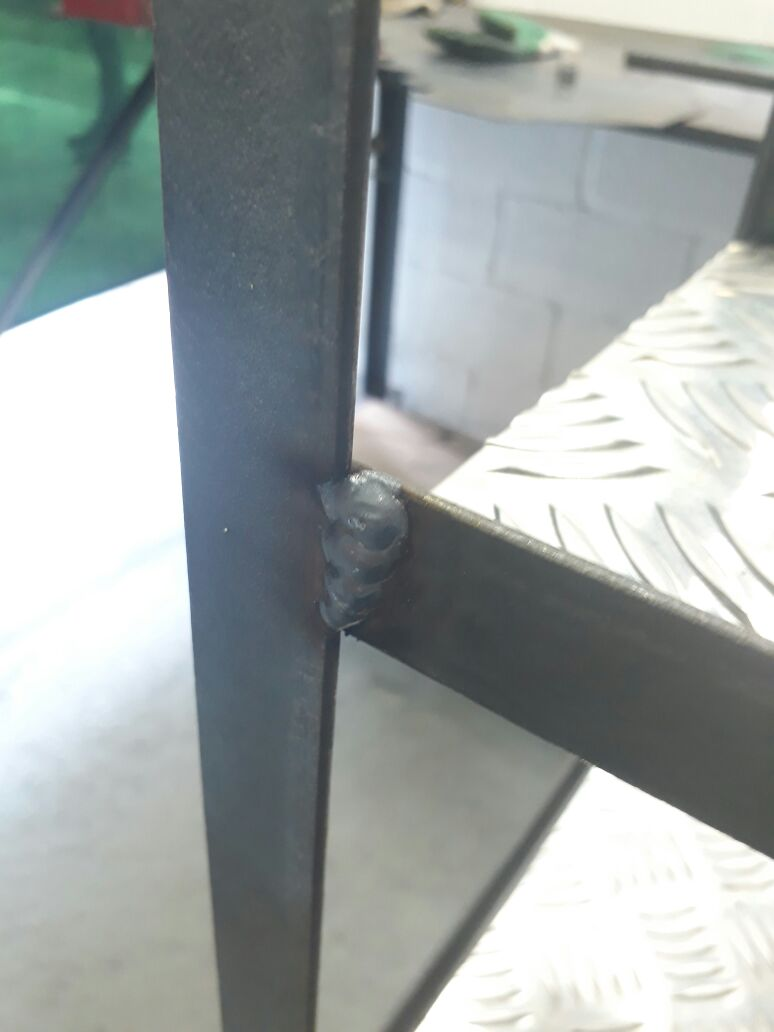
\includegraphics[scale= 0.2]{figuras/estrutura/solda-realizada.jpg}
    \caption{Solda realizada na estrutura. Fonte: Própria.}
    \label{modelagem}
  \end{figure}

  Após a soldagem de todas as bases, as 4 vigas principais da estrutura foram unidas as 
  bases de forma que fosse possível erguer a estrutura. Foi iniciado, então, o processo 
  de soldagem dos subníveis menores, referentes aos componentes eletrônicos e de automação.

  \begin{figure}[H]
    \centering
    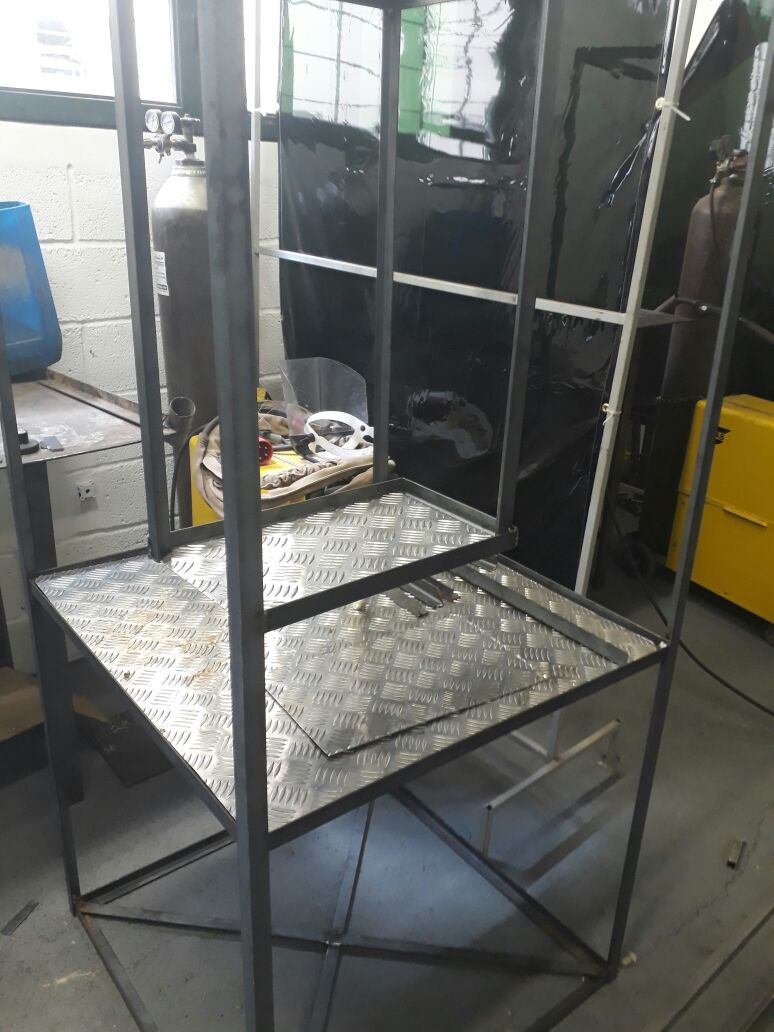
\includegraphics[scale= 0.3]{figuras/estrutura/frame-principal-soldagem.jpg}
    \caption{Frame principal após o término da soldagem. Fonte: Própria.}
    \label{modelagem}
  \end{figure}

  Assim que terminados os processos de soldagem as placas metálicas foram fixadas ao frame. 
  A fixação escolhida foi uma fita de alta resistência da 3m. A utilização da fita evitou o
  exagero no uso de parafusos e soldagem, o que reduziu custo e facilitou qualquer manutenção 
  eventual que tenha de ser realizada na estrutura.

  Todo o acabamento final, que é responsável por toda a estética do equipamento, 
  foi feito com chapas de alumínio cortadas e dobradas. 

  É importante ressaltar que a equipe de estrutura ficou responsável pelo mecanismo de 
  acionamento da base que inclina o copo. Foi projetado um mecanismo simples de biela-manivela 
  fabricado através de impressão 3d. A manivela eh rotacionada por um motor de passo que empurra a 
  biela contra a base de forma que ela pivota em seu suporte superior.

  \begin{figure}[H]
    \centering
    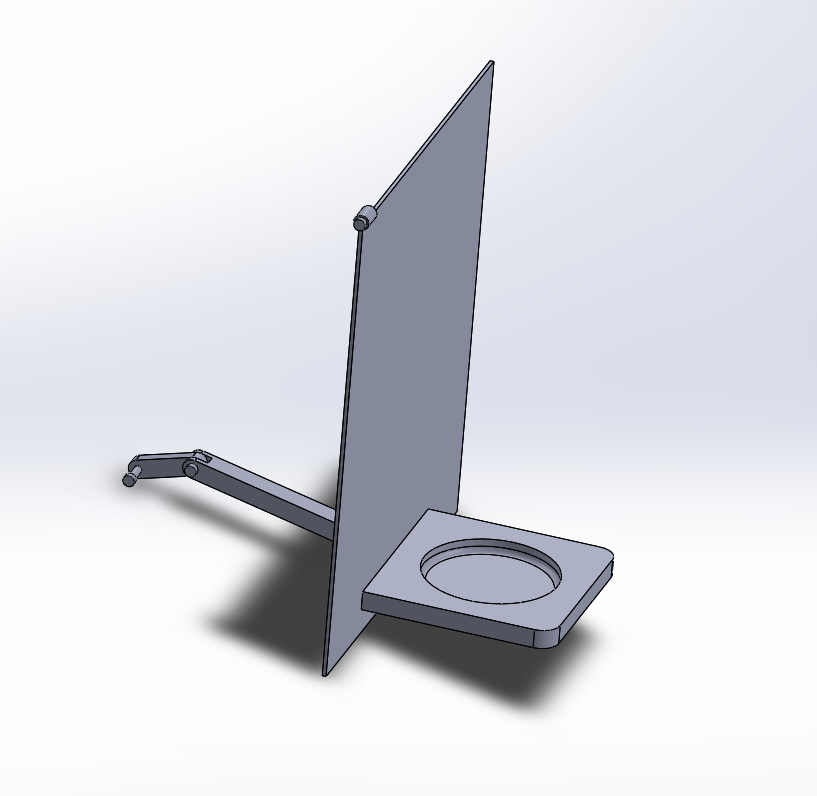
\includegraphics[scale= 0.5]{figuras/estrutura/mecanismo-inclinacao.png}
    \caption{Mecanismo de inclinação do chopp. Fonte: Própria.}
    \label{modelagem}
  \end{figure}



  
